\section{Methodology}\label{methodology}

\subsection{Overview of types of
methodology}\label{overview-of-types-of-methodology}

\subsubsection{Development Styles}\label{development-styles}

\paragraph{Rapid Applications Development
(RAD)}\label{rapid-applications-development-rad}

By producing prototypes of the software quickly customers are able to
test and provide feedback as the software is developed. This is useful
as often requirements change and it's common for developers to produce
software that isn't actually what the customer wanted, by providing them
with quickly developed prototypes if the software isn't what they wanted
or they would like to make changes the time impact has been reduced.
This is especially compared to other methodologies such as waterfall
where the entire project is completed start to finish with the aim of
providing the completed software at the end.

RAD I feel is not suited to my project as I am developing software that
I know the requirements for and so will have no issues with changes to
the requirements. RAD however is more of an encompassing methodology
which is built upon fast paced development strategies.

\paragraph{Agile}\label{agile}

Is not a methodology but instead seeks for alternative project
management style. Originally project management was slow to adapt to
changes with user review coming in late stages of development. Agile
however aims for incremental development with regular feedback.
\parencite{agile}

The most popular form of agile development is the Scrum
\parencite{agile} scrum is suited towards small teams and requires close
involvement by the product owner to provide regular feedback and review.
There are other forms such as; - Extreme Programming, this a more
disciplined approach to develop high-quality software quickly and
involves continuous testing and planning - Crystal, aims to be
lightweight and a highly adaptable methodology and encompasses variants
that can be better suited for different team sizes, project priorities
and on system criticality. \parencite{agilemethods} - Dynamic Systems
Development Method (DSDM), is a very early methodology to come from the
RAD movement in the early 90's and it focuses on the 80/20 model where
the useful 80\% of the system that can be produced in 20\% of the time,
essentially leaving more complex aspects to the later stages of
development. \parencite{agilemethods}

Agile and the use of scrum development would appear to be very well
suited to my project as it will allow for rapid development of features
in my application, by quickly developing the base functionality and
being able to obtain feedback from my supervisor before expanding to the
other features would be extremely helpful and would prevent wasted time
if I need to make changes.

\paragraph{Lean}\label{lean}

Much like scrum and other agile methodologies aims to produce software
quickly and involves close coordination with the product owner, where
lean varies is that it wants to reduce waste by selecting the most
valuable features required. Lean also works well for groups of small
teams or individuals as it has a focus on decision making authority
which has been shown to be more efficient than hierarchical flow control
\parencite{agilemethods}.

\paragraph{Waterfall}\label{waterfall}

Is not an RAD strategy and instead focuses on phases such as;
requirement gathering, analyses, development and testing. Each phase is
completed entirely before moving onto the next phase and is often
depicted by the phases flowing steadily downwards resembling a
waterfall.

Waterfall is slow to changes and delays in early phases can have a large
impact on later phases and can easily end up missing the deadline.
Waterfall is often easier to understand as it's a linear process and due
to phases being performed to completion documentation is often more
thorough than in agile methodologies \parencite{agilevswaterfall}.

Due to the slower nature of waterfall I don't feel it would be ideal for
my project, although it's easier to plan and performing agile
development will lead to a greater challenge in documentation, the
flexibility provided by agile would suit my needs greater than such a
rigid method like waterfall.

\paragraph{Spiral}\label{spiral}

The spiral model is based on the incremental model and consists of four
phases; Planning, risk analysis, engineering and evaluation
\parencite{spiral}. A project will go through each phase multiple times
in an iterative process or spirals. This is very well illustrated in the
figure below.

\begin{figure}[htbp]
\centering
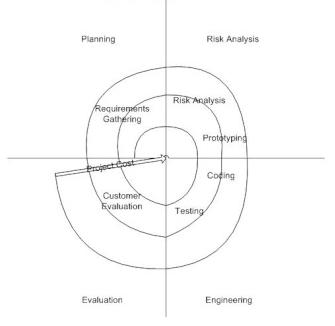
\includegraphics{../../Images/Spiral-model.jpg}
\caption{Spiral model diagram \parencite{spiral}}
\end{figure}

Each spiral builds upon the previous spirals and due to the repetition
of the four stages risk analysis is more rigorous compared to other
methodologies.

Due to how the spiral method works I don't feel it would be suited for
my project as it requires multiple passes through each phase and as my
project is relatively small and has a limited deadline I feel too much
time would be spent on planning and risk analysis reducing my time
developing and testing my application.

\paragraph{Time Boxing}\label{time-boxing}

Involves strict deadlines rather than goals. By developing up to the
agreed upon time and evaluating progress this can allow for steadier
development and a set time in mind which provides a deadline for
development.

Evaluating at the end of the time frame can show struggles in the
development process and provides the ability to address them rather than
simply spending more time to complete the goal.

There are issues with this method of development as it is difficult to
estimate the time required to complete a task and so underestimating the
time box will regularly involve assessing unfinished work. Potentially
worse however is over estimating as this would allow adequate time to
complete goals but will not help in identifying issues with development
and will also result in a more relaxed time scale that could easily miss
deadlines.

This would be very useful in my project as it will allow me to estimate
a time frame for each feature of my application, allowing me to reflect
on my progress as well as for my scheduled meeting with my supervisor.

\subsection{Choice of methodology}\label{choice-of-methodology}

After assessing the various forms of project methodologies I have
decided to use an agile methodology most notably the Lean methodology as
this will provide me the ability to develop core functionality in a fast
pace and add other features time permitting. To assist my development I
will also be using time boxing to allocate time for my applications
functions and allow me to perform regular performance reviews so I can
identify time sinks and other issues to allow me to manage them.
